\chapter{Technique Overview}\label{ch:research}
The objective is to create an overview of techniques in the field which may be used to solve the
problem detailed in Chapter~\ref{ch:problem}.
According to the methodology detailed in~\ref{se:methodology}, first a taxonomy is introduced
which facilitates the analysis and comparison of techniques.
The subsequent search for literature which lays the foundation for an overview over current research
is documented.
Lastly, the advances in the field are placed in the correct position and analyzed.

\section{Taxonomy of Pipeline Steps}
Before getting into current research level, a base of knowledge about the field has to be layed.
A taxonomy is created for this which is useful to classify and give context to innovations in the
field.
\begin{figure}[b]
    \centering
    \resizebox{0.4\linewidth}{!}{%
\begin{tikzpicture}[
    every node/.style={draw=black,thin,anchor=west, minimum height=2.5em},
    lroot/.style={%
        edge from parent fork down,
        level distance=0.5cm,
        text centered, text width=3cm},
    lone/.style={%
        text centered, text width=3cm,
        level distance=0.5cm},
    ltwo/.style={%
        rounded corners,
        grow=down, xshift=-0.8cm,
        text centered, text width=3cm,
        edge from parent path={(\tikzparentnode.205) |- (\tikzchildnode.west)}},
    level1/.style ={level distance=1.2cm},
    level2/.style ={level distance=2.4cm},
    level3/.style ={level distance=3.6cm},
    level4/.style ={level distance=4.8cm},
    level5/.style ={level distance=6.0cm},
    level 1/.style={sibling distance=4cm},
    level 1/.append style={level distance=1.5cm},
]
%   \draw[help lines] (0,0) grid (4,3);

    % lroot
    \node[anchor=south,lroot]{E2E}
    [edge from parent fork down]
            child{node [lone] {2-step}
                child[ltwo,level1] {node {STD \\ }}
                child[ltwo,level2] {node {STR with \\ cropped images}}
            }
            child{node [lone] {2-stage}
                child[ltwo,level1] {node {STD}}
                child[ltwo,level2] {node {STR with \\ feature maps}}
            };
        %

\end{tikzpicture}
}%

    \caption{Different E2E Pipelines\label{fig:e2e-pipelines}}
\end{figure}
The partition of tasks and categorization of approaches is conducted according to overview literature
such as~\cite{long_scene_2021,chen_text_2021,cong_comparative_2019} and related research in the
field such as~\cite{qiao_text_2021,sheng_centripetaltext_2021,liu_accurate_2020,deng_pixellink_2018}.
To create the overview the necessary steps in the process of \ac{STS} need to be highlighted,
from preprocessing to classifying the identified
text~\citep{long_scene_2021, sourvanos_challenges_2018}.
The ways in which the respective issues for the steps are solved are identified from literature,
listed and explained alongside.
Figure~\ref{fig:e2e-pipelines} shows two pipelines categories for end to end \ac{STS}
approaches~\citep{long_scene_2021}.
\ac{STD} and \ac{STR} only incorporate a part of \ac{STS}, while end to end approaches
incorporate both \ac{STD} and \ac{STR} techniques to solve
\ac{STS}~\citep{long_scene_2021,ghosh_visual_2017,chen_text_2021}.
Therefore this section will first discuss the two parts, to then later combine them.

For \ac{STD} two main categories of approaches can be identified: segmentation based and \ac{BB}
regression based (see
Figure~\ref{fig:STD-pipelines})~\citep{long_scene_2021,sheng_centripetaltext_2021,liu_accurate_2020}.
\begin{figure}[ht]
    \centering
    \resizebox{0.6\linewidth}{!}{%
\begin{tikzpicture}[
    every node/.style={draw=black,thin,anchor=west, minimum height=2.5em},
    lroot/.style={%
        edge from parent fork down,
        level distance=0.5cm,
        text centered, text width=3cm},
    lone/.style={%
        text centered, text width=3cm,
        level distance=0.5cm},
    ltwo/.style={%
        text centered, text width=3cm,
        level distance=0.5cm},
    lthree/.style={%
        rounded corners,
        grow=down, xshift=-0.8cm,
        text centered, text width=3cm,
        edge from parent path={(\tikzparentnode.205) |- (\tikzchildnode.west)}},
    level1/.style ={level distance=1.2cm},
    level2/.style ={level distance=2.4cm},
    level3/.style ={level distance=3.6cm},
    level4/.style ={level distance=4.8cm},
    level5/.style ={level distance=6.0cm},
    level 1/.style={sibling distance=8cm},
    level 1/.append style={level distance=1.5cm},
    level 2/.style={sibling distance=4cm},
    level 2/.append style={level distance=1.5cm},
]
%   \draw[help lines] (0,0) grid (4,3);

    % lroot
    \node[anchor=south,lroot]{STD}
    [edge from parent fork down]
        child{node [lone] {BB regression}
            child{node [ltwo] {One-stage}
                child[lthree,level1] {node {Feature \\ extraction}}
                child[lthree,level2] {node {Text instance \\ localization}}
                child[lthree,level3] {node {Result \\ filtering}}
            }
            child{node [ltwo] {Two-stage}
                child[lthree,level1] {node {Feature \\ extraction}}
                child[lthree,level2] {node {Text region \\ localization}}
                child[lthree,level3] {node {Localization \\ readjustment}}
                child[lthree,level4] {node {Result \\ filtering}}
            }
        }
        child{node [lone] {Segmentation \\ based}
            child[lthree,level1] {node {Feature \\ extraction}}
            child[lthree,level2] {node {Sub-component \\ segmentation}}
            child[lthree,level3] {node {Text \\ reconstruction}}
        };
\end{tikzpicture}
}%

    \caption{Different STD Pipelines\label{fig:STD-pipelines}}
\end{figure}
The regression based category draws heavy inspiration from the field of object
detection~\citep{long_scene_2021,liu_accurate_2020}.
This is only natural as text detection can be seen as a type of object
detection~\citep{liu_accurate_2020,long_scene_2021}.
For object detection inspired \ac{STD} there are two methods: one stage and two
stage~\citep{long_scene_2021}.
Both localize text instances as a whole (in the form of a
\ac{BB})~\citep{long_scene_2021,sheng_centripetaltext_2021}.
One stage approaches are modelled after~\cite{liu_ssd_2016}, Single Shot MultiBox
Detector (SSD) and~\cite{redmon_you_2016}, You Only Look Once (YOLO).
They have in comon that \acp{BB} are regressed once and not changed or optimized
afterwards~\citep{redmon_you_2016,liu_ssd_2016}, as opposed to the \ac{ROI} based approach with two
stages~\citep{girshick_rich_2014}.
\begin{figure}[ht]
    \centering
    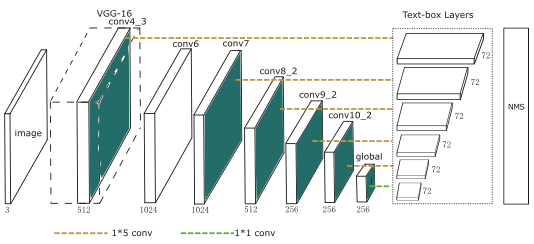
\includegraphics[width=0.8\textwidth]{img/STD-seg-free-Liao-TextBoxes-2017.png}
    \caption[One stage, BB regression based STD architecture]{%
        Example for a one stage, BB regression based STD
        architecture~\citep{liao_textboxes_2017}\label{fig:STD-segfree-ssd}
    }
\end{figure}
The basic approach is explained with the example of~\cite{liao_textboxes_2017} (see
Figure~\ref{fig:STD-segfree-ssd}) which is based on SSD.\
Note that the approach is modeled to recognize horizontal text instances~\citep{liao_textboxes_2017}.
It uses convolutional network inspired by the VGG architecture (blocks of: two or
three $3\times3$ conv layers followed by a $2\times2$ max pooling layer with stride 2) for feature
extraction~\citep{liao_textboxes_2017,simonyan_very_2015}.
Note that the spatial padding added for convolution ensures that spatial dimensions are
preserved~\citep{simonyan_very_2015}.
Afterwards come additional layers which continuously downsample.
The output of six of them is separately used as feature maps for \ac{BB}
regression~\citep{liao_textboxes_2017}.
The downsampling and \ac{BB} regression for different layers helps detect text instances of different
scales~\citep{liu_ssd_2016}.
Each spatial location on the feature map can be traced back to a region on the input
image~\citep{long_scene_2021}.
The \ac{BB} regression is carried out by six convolutional text-box layers which predict how
certain ($c_1,c_2$) the prediction is a text instance or background and where the text instance
is ($x,y,w,h$).
Note that the output is not the location of a \ac{BB} but the offset to the
respective anchor box~\citep{liao_textboxes_2017,long_scene_2021}.
Anchor boxes are predefined to give bias towards sizes and aspect ratios of
text~\citep{liao_textboxes_2017}.
The text-box layers are the difference to the SSD approach for normal object
detection~\citep{liao_textboxes_2017,liu_ssd_2016}.
These layers use $1\times5$ filters to adjust to larger aspect ratios~\citep{liao_textboxes_2017}.
Each text-box layer has 72 filters (12 anchor boxes $\cdot$ 6 values per prediction), the filters
are slided accross the input features generating 12 predicted \ac{BB} per
position~\citep{liao_textboxes_2017}.
The \acp{BB} of all layers are then subjected to the process of \ac{NMS} to filter out the best
\ac{BB} for each possible text instance~\citep{liao_textboxes_2017}.
For this \ac{NMS} is used: of all detections which overlap more than a threshhold $\phi$ only the
with the highest confidence score ($c$) is kept~\citep{hosang_learning_2017}.

The R-CNN which builds the foundation for \ac{ROI} based text detection, was introduced
by~\cite{girshick_rich_2014} and improved by~\cite{girshick_fast_2015} (Fast
R-CNN),~\cite{ren_faster_2015} (Faster R-CNN) and~\cite{he_mask_2018} (Mask R-CNN).
Note that 2-stage methods are fully differentiable and thus end to end trainable since
Faster R-CNN (like 1-stage methods)~\citep{ren_faster_2015,long_scene_2021}.
The two stages consist of: \ac{ROI} regression, \ac{BB}
adjustments~\citep{jiang_r2cnn_2017, ren_faster_2015}.
The \ac{STD} approach introduced by~\cite{jiang_r2cnn_2017} (see Figure~\ref{fig:STD-segfree-rcnn})
uses Faster R-CNN.%
Unlike the previous approach, the architecture is designed to detect multioriented text
instances~\citep{jiang_r2cnn_2017,liao_textboxes_2017}.
\begin{figure}[ht]
    \centering
    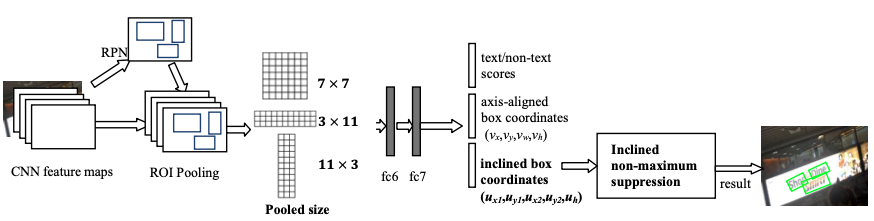
\includegraphics[width=0.8\textwidth]{img/STD-seg-free-Jiang-R2CNN-2017.png}
    \caption[Two stage, BB regression based STD architecture]{%
        Example for a two stage, BB regression based STD
        architecture~\citep{jiang_r2cnn_2017}\label{fig:STD-segfree-rcnn}
    }
\end{figure}
Like with the one stage approach, the two stage approach starts with feature extraction from the
image with a convolutional layers~\citep{jiang_r2cnn_2017}.
Feature extraction \ac{CNN} is again inspired by the VGG architecture~\citep{jiang_r2cnn_2017},
like in the previous approach.
The generated feature map is used by a \ac{RPN}.
Like with the previously explained approach, the feature maps are used to regress the offset
respective to bounding boxes.
The bounding boxes are still axis aligned at this point~\citep{jiang_r2cnn_2017}.
In contrast to the previous SSD based approach, only one feature map is used in conjunction with
\ac{BB} regression~\citep{jiang_r2cnn_2017}.
The \ac{RPN} from Faster R-CNN is adjusted to use smaller scale anchor boxes to adapt to
text~\citep{jiang_r2cnn_2017}.
Note that R-CNN and Fast-RCNN used the slower Sequential Search algorithm instead of an
\ac{RPN}~\citep{girshick_rich_2014,girshick_fast_2015}.
The resulting \acp{BB} are called \acp{ROI}~\citep{ren_faster_2015,jiang_r2cnn_2017}.
They are used for \ac{ROI} pooling in conjunction with the original feature maps.
This layer uses max pooling to convert the spatial features corresponding to the location of the
\ac{ROI} to a small feature map~\citep{girshick_fast_2015}.
In the case of this example, \ac{ROI} pooling is used to create three feature maps with different
aspect ratios ($7\times7, 3\times11, 11\times3$) which are concatenated for the next
step~\citep{jiang_r2cnn_2017}.
The second stage is to predict a confidence score (text, background) for each \ac{ROI} and to
refine them by regressing values ($x_1,y_1,x_2,y_2,h$) that allow for inclined boxes to account for
rotated text~\citep{jiang_r2cnn_2017}.
At last the resulting \acp{BB} are filtered by inclined \ac{NMS} which is adjusted to the
incline \acp{BB}~\citep{jiang_r2cnn_2017}.

The basis for the segmentation based methods is the fact that every part of the text instance can
be used to verify that there is text~\citep{long_scene_2021}.
Because of this, sub-text components can be detected separately and then used to re-construct a text
instance~\citep{long_scene_2021}.
Segmentation based methods can roughly be summed up in two categories: pixel based and component
based~\citep{long_scene_2021}.
Like with \ac{BB} regression based methods, example architectures are explained in order to
describe their categories more clearly.
\begin{figure}[ht]
    \centering
    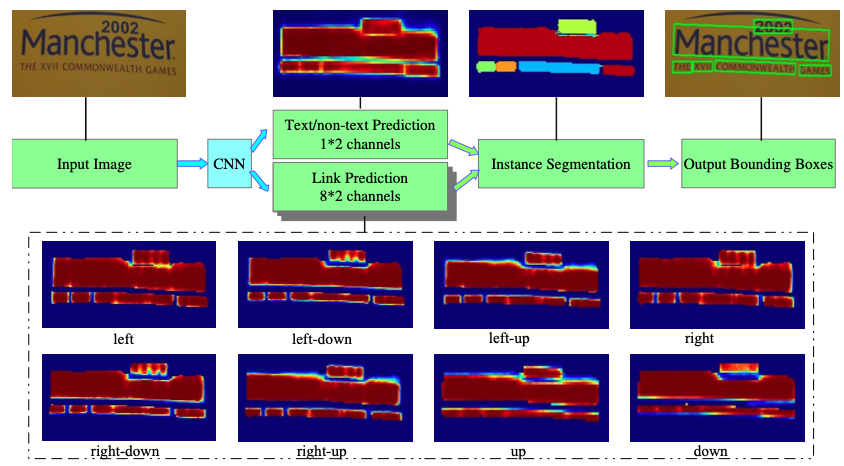
\includegraphics[width=0.7\textwidth]{img/STD-seg-based-architecture-Deng-PixelLink-2018.png}
    \caption[Pixel, segmentation based STD architecture]{%
        Example for a pixel, segmentation based STD
        architecture~\citep{deng_pixellink_2018}\label{fig:STD-segbased-pixel-architecture}
    }
\end{figure}
The paper~\cite{deng_pixellink_2018} introduced a pixel based \ac{STD} approach.
Figure~\ref{fig:STD-segbased-pixel-architecture} shows its pipeline.
First segmentation creates a dense segmentation maps which are used to then segregate different
instances of text~\citep{deng_pixellink_2018}.
Figure~\ref{fig:STD-segbased-pixel-CNN} shows the \ac{CNN} structure for feature extraction
(until conv5) which is basically VGG architecture with the fully connected layers exchanged with
another convolutional stage~\citep{deng_pixellink_2018}.
% FIXME: essentially CNN encoder decoder~\citep{badrinarayanan_segnet_2017}
\begin{figure}[ht]
    \centering
    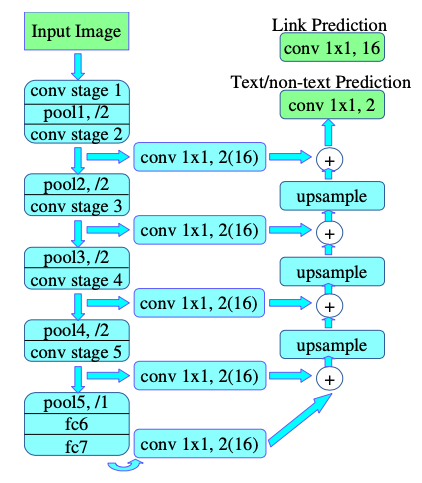
\includegraphics[width=0.35\textwidth]{img/STD-seg-based-CNN-Deng-PixelLink-2018.png}
    \caption[Feature extractor and prediction head for pixel segmentation]{%
        PixelNet CNN feature extractor with head structure for pixel
        segmentation\label{fig:STD-segbased-pixel-CNN}
    }
\end{figure}
The feature extraction followed by two heads which either predict text/non-text or
links~\citep{deng_pixellink_2018}.
The structure which combines downsampled feature maps with later upsampled ones is inspired
by~\cite{long_fully_2015}.
Continuous downsampling and and combining those layers with later, upsampled layers helps
to combine coarse, higher level information with fine, lower level
information~\citep{long_fully_2015}.
The upsampling is performed with bilinear interpolation~\citep{deng_pixellink_2018}.
Depending on which head is used, the $1\times1$ convolution layers either have 2 or $2\cdot8$ filters.
Counted together, the model has 18 output channels~\citep{deng_pixellink_2018}.
The $1\times1$ convolution layers are also used for upsampling (deconvolution,
see~\cite{noh_learning_2015,long_fully_2015} for an in depth explanation)
for the feature combination~\citep{deng_pixellink_2018}.
2 filters are used to predict text/non-text for each pixel, while the other 16 filters predict
the links~\citep{deng_pixellink_2018}.
The text/non-text head essentially performs semantic segmentation, that is to categorize each
pixel to its type~\citep{deng_pixellink_2018}.
For every neighbor there is a negative and a positive score.
A pixel has eight neighbors: left, left-down, left-up, right, right-down, right-up, up, down.
Each of the $2\cdot8$ filters is responsible for a neighbor link~\citep{deng_pixellink_2018}.
After both links and text/non-text pixels have been predicted, they are combined for instance
segmentation~\citep{deng_pixellink_2018}.
The link layers are used to indicate whether two text pixels are grouped together an thus belong to
the same instance~\citep{deng_pixellink_2018}.
The output is a dense prediction map with the same spatial structure as the input
image~\citep{deng_pixellink_2018}.
A bounding box can then be extracted by laying minimum area rectangles over the
instances~\citep{deng_pixellink_2018}.

The second segmentation based category for \ac{STD} segments components which are local regions of
text that can overlap one or more characters~\citep{long_scene_2021}.
\begin{figure}[ht]
    \centering
    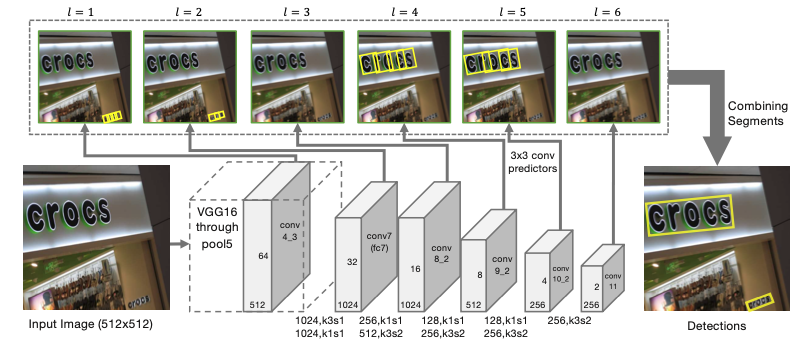
\includegraphics[width=0.9\textwidth]{img/STD-seg-based-architecture-Shi-Detecting-2017.png}
    \caption[Sub-component, segmentation based STD architecture]{%
        Example for a sub-component, segmentation based STD
        architecture~\citep{shi_detecting_2017}\label{fig:STD-segbased-component-architecture}
    }
\end{figure}
The architecture (see Figure~\ref{fig:STD-segbased-component-architecture})
from~\cite{shi_detecting_2017} is used as an example for this category.
Like the one-stage, \ac{BB} regression based \ac{STD} approach, the feature extraction \ac{CNN} of
this approach is taken from SSD and thus VGG, the difference is reflected in the prediction
layers~\citep{shi_detecting_2017,liu_ssd_2016,simonyan_very_2015}.
Instead of detecting whole \acp{BB}, the networks predicts both subcomponents and links at multiple
scales~\citep{shi_detecting_2017}.
The convolutional prediction is carried out with seven $3\times3$ filters followed by a softmax
nonlinearity for normalization.
The segments are given by the values $x_s,y_s,w_s,h_s,\theta_s$ which offset an anchor box as well
as confidence scores $c_1,c_2$~\citep{shi_detecting_2017}.
Links are used to combine the segments and are accordingly used to separate neraby
words~\citep{shi_detecting_2017}.
Like with $c_1,c_2$, for every neighbor and cross layer neighbor a positive and a negative value
is predicted~\citep{shi_detecting_2017}.
\begin{figure}[ht]
    \centering
    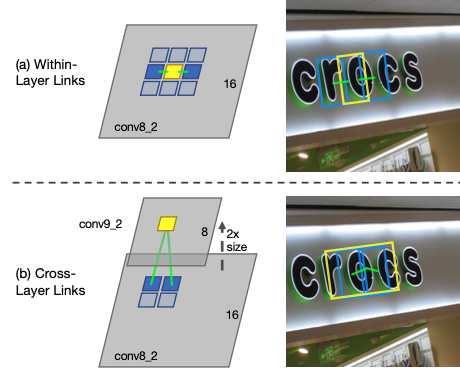
\includegraphics[width=0.5\textwidth]{img/STD-seg-based-links-Shi-Detecting-2017.png}
    \caption[Predicting links for segmentation based STD]{%
        Visualization for prediction of links within and cross layers for segmentation based
        STD~\citep{shi_detecting_2017}\label{fig:STD-segbased-component-links}
    }
\end{figure}
% XXX: are equations really needed?
Within layer links are predicted for the neighbors of a space in the predicted feature map
(see Figure~\ref{fig:STD-segbased-component-links} (a),
Equation~\ref{eq:STD-segbased-subcomp-same-layer})~\citep{shi_detecting_2017}.
\begin{equation}\label{eq:STD-segbased-subcomp-same-layer}
    \mathcal{N}_{s^{x,y,l}}^w =
        \frac{{\{s^{(x',y',l)}\}}_{x-1\leq x'\leq x+1,y-1\leq y'\leq y+1}}{s^{(x,y,l)}}
\end{equation}
The cross layer links on the other hand are predicted by using the 4 cross layer neighors of the
feature map of the preceding predictor~\citep{shi_detecting_2017}.
(see Figure~\ref{fig:STD-segbased-component-links} (b),
Equation~\ref{eq:STD-segbased-subcomp-cross-layer})~\citep{shi_detecting_2017}.
\begin{equation}\label{eq:STD-segbased-subcomp-cross-layer}
    \mathcal{N}_{s^{x,y,l}}^c = {\{s^{(x',y',l-1)}\}}_{2x\leq x'\leq 2x+1,2y\leq y'\leq 2y+1}
\end{equation}
These cross layer links are used to connect segments on different scales~\citep{shi_detecting_2017}.
The network architecture designed so that the preceding feature map is twice the size (spatial
dimensions) of the current which is necessary to extract the right
locations~\citep{shi_detecting_2017}.
Before reconstruction the text instances, segments are filtered by their confidence
scores~\citep{shi_detecting_2017}.
To reconstruct, the predictions are taken as a graph: segments are nodes, links are edges.
Depth-first search is applied to the graph to find connected components and thus text
instances~\citep{shi_detecting_2017}.

For \ac{STR} two main categories of approaches can be identified: segmentation based and
encoder decoder based (see Figure~\ref{fig:str-pipelines})~\citep{chen_text_2021}.
\begin{figure}[h]
    \centering
    \resizebox{0.6\linewidth}{!}{%
\begin{tikzpicture}[
    every node/.style={draw=black,thin,anchor=west, minimum height=2.5em},
    lroot/.style={%
        edge from parent fork down,
        level distance=0.5cm,
        text centered, text width=3cm},
    lone/.style={%
        text centered, text width=3cm,
        level distance=0.5cm},
    ltwo/.style={%
        text centered, text width=3cm,
        level distance=0.5cm},
    lthree/.style={%
        rounded corners,
        grow=down, xshift=-0.8cm,
        text centered, text width=3cm,
        edge from parent path={(\tikzparentnode.205) |- (\tikzchildnode.west)}},
    level1/.style ={level distance=1.2cm},
    level2/.style ={level distance=2.4cm},
    level3/.style ={level distance=3.6cm},
    level4/.style ={level distance=4.8cm},
    level5/.style ={level distance=6.0cm},
    level 1/.style={sibling distance=6cm},
    level 1/.append style={level distance=1.5cm},
    level 2/.style={sibling distance=5cm},
    level 2/.append style={level distance=1.5cm},
]
%   \draw[help lines] (0,0) grid (4,3);

    % lroot
    \node[anchor=south,lroot]{STR}
    [edge from parent fork down]
        child{node [ltwo] {Segmentation \\ based}
            child[lthree,level1] {node {Image \\ preprocessing}}
            child[lthree,level2] {node {Feature \\ extraction}}
            child[lthree,level3] {node {Character \\ segmentation}}
            child[lthree,level4] {node {Character \\ recognition}}
        }
        child{node [lone] {Segmentation \\ free}
            child{node [ltwo] {CTC}
                child[lthree,level1] {node {Image \\ preprocessing}}
                child[lthree,level2] {node {Feature \\ extraction}}
                child[lthree,level3] {node {Sequence \\ modelling}}
                child[lthree,level4] {node {CTC rule \\ application}}
            }
            child{node [ltwo] {Encoder-Decoder}
                child[lthree,level1] {node {Image \\ preprocessing}}
                child[lthree,level2] {node {Feature \\ extraction}}
                child[lthree,level3] {node {Sequence \\ modelling}}
                child[lthree,level4] {node {Sequence \\ decoder}}
            }
        };
\end{tikzpicture}
}%

    \caption{Different STR Pipelines\label{fig:str-pipelines}}
\end{figure}
Segmentation based approaches for \ac{STR} are similar to segmentation based approaches for \ac{STD}.
After feature extraction, the subtext components (characters for \ac{STR}) are
segmented~\citep{chen_text_2021}.
Instead of reconstructing a \ac{BB}, the characters are classified to recognize the
text and are then used to form the text instance~\citep{chen_text_2021}.
Because of their similarity to \ac{STD} and the recent domiance of encoder decoder based
approaches~\citep{chen_text_2021,long_scene_2021}, only the later will be explained in detail with
examples.
The approach from~\cite{wan_textscanner_2020} can be used as an example, should the reader feel the
need to read up on segmentation based methods for \ac{STD} that do not include an encoder decoder
mechanism in the prediciton stage.
\begin{figure}[h]
    \centering
    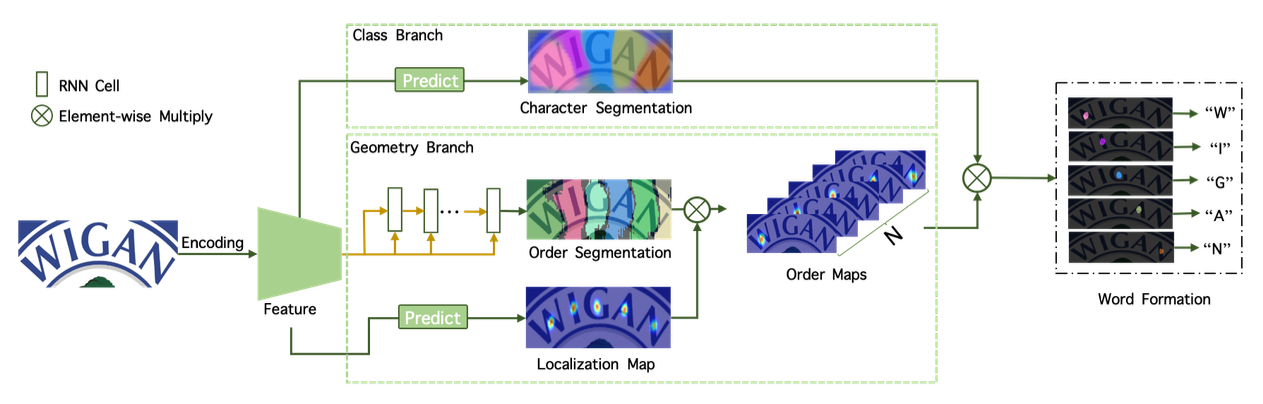
\includegraphics[width=0.8\textwidth]{img/STR-seg-based-wan-textscaner-2020.png}
    \caption[Segmentation based STR architecture]{%
        Example for segmentation based STR
        architecture~\citep{wan_textscanner_2020}\label{fig:STR-segbased-architecture}
    }
\end{figure}
The approach adds a geometry branch parallel to the charcater segmentation which helps with with
putting the identified characters in the right sequence (see
Figure~\ref{fig:STR-segbased-architecture})~\citep{wan_textscanner_2020}.

Encoder-decoder based approaches can again be divided into \ac{CTC} based and attention based
approaches (see
Figure~\ref{fig:STR-segbased-architecture})~\citep{long_scene_2021,cong_comparative_2019}.
\begin{figure}[h]
    \centering
    \resizebox{0.8\linewidth}{!}{\scriptsize%
\begin{tikzpicture}[%
    hid/.style 2 args={%
        rectangle split,
        rectangle split horizontal,
        draw=#2,
        rectangle split parts=#1,
        fill=#2!20,
        outer sep=1mm
    }
]
    % draw input nodes
    \foreach \i [count=\step from 1] in {the,blue,house,{{$<$bos$>$}}}
    \node (i\step) at (2*\step, -2) {\i};
    % draw output nodes
    \foreach \t [count=\step from 4] in {das,blaue,Haus,{{$<$eos$>$}}} {
        \node[align=center] (o\step) at (2*\step, +2.75) {\t};
    }
    % draw embedding and hidden layers for text input
    \foreach \step in {1,...,3} {
        \node[hid={3}{red}] (h\step) at (2*\step, 0) {};
        \node[hid={3}{red}] (e\step) at (2*\step, -1) {};
        \draw[->] (i\step.north) -> (e\step.south);
        \draw[->] (e\step.north) -> (h\step.south);
    }
    % draw embedding and hidden layers for label input
    \foreach \step in {4,...,7} {
        \node[hid={3}{yellow}] (s\step) at (2*\step, 1.25) {};
        \node[hid={3}{blue}] (h\step) at (2*\step, 0) {};
        \node[hid={3}{blue}] (e\step) at (2*\step, -1) {};
        \draw[->] (e\step.north) -> (h\step.south);
        \draw[->] (h\step.north) -> (s\step.south);
        \draw[->] (s\step.north) -> (o\step.south);
    }
    \draw[->] (h3.east) edge[->,out=330,in=200] (h5.south);
    \draw[->] (h3.east) edge[->,out=330,in=190] (h6.south);
    \draw[->] (h3.east) edge[->,out=330,in=180] (h7.south);
    % edge case: draw edge for special input token
    \draw[->] (i4.north) -> (e4.south);
    % draw recurrent links
    \foreach \step in {1,...,6} {
        \pgfmathtruncatemacro{\next}{add(\step,1)}
        \draw[->] (h\step.east) -> (h\next.west);
    }
    % draw predicted-labels-as-inputs links
    \foreach \step in {4,...,6} {
        \pgfmathtruncatemacro{\next}{add(\step,1)}
        \path (o\step.north) edge[->,out=45,in=225] (e\next.south);
    }
\end{tikzpicture}
}
%
    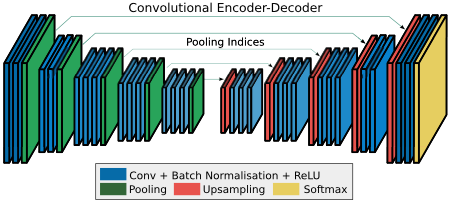
\includegraphics[width=0.7\textwidth]{img/Encoder-Decoder-Conv-Badrinarayanan-SegNet-2017.png}
    \caption[Encoder decoder architectures]{%
        Encoder decoder architecture with \acp{RNN} and \acp{CNN}
        respectively~\citep{cho_learning_2014,badrinarayanan_segnet_2017}\label{fig:enc-dec}
    }
\end{figure}
The \ac{RNN} encoder decoder can be used to transform a sequence of variable length into another
sequence with different variable length~\citep{cho_learning_2014}.
The encoder processes the input sequence and crafts a representation vector that encodes information
and context for the whole input sequence which can then be used for every time step in the decoder
network~\citep{cho_learning_2014}.
The \ac{CNN} encoder decoder architecture was already introduced with the pixel-level,
segmentation example for \ac{STD} (see
Figure~\ref{fig:STD-segbased-pixel-CNN})~\citep{deng_pixellink_2018}.
Continuous downsampling and and combining those layers with later, upsampled layers helps to generate
context for image features by combining coarse, higher level information with fine, lower level
information~\citep{long_fully_2015,badrinarayanan_segnet_2017}.
Often preprocessing steps are performed to remove distortions, rectify curved text,
remove disruptive background, improve resolutions or recover degraded text.
Especially rectifying curved text (see Figure~\ref{fig:STN-application}) with the help of
thin-plate spines~\citep{bookstein_principal_1989} or spatial transformer
networks~\citep{jaderberg_spatial_2015} shows great improvement for \ac{STR}
performance~\citep{long_scene_2021,chen_text_2021}.
\begin{figure}[h]
    \centering
    
\includegraphics[width=0.4\textwidth]{img/STN-result-Liu-STAR-2016.png}
    \caption[Text rectification application]{%
        Application of spatial transformer network to rectify curved
        text~\citep{liu_star-net_2016}\label{fig:STN-application}
    }
\end{figure}
For feature extraction different \ac{CNN} architectures can be chosen.
The tradeoff between performance and memory \& computation cost determines what \ac{CNN} should be
chosen~\citep{chen_text_2021}.
An example for a deep and powerful \ac{CNN} are ResNets~\citep{he_deep_2015} which are often used
for benchmark purposes~\citep{chen_text_2021,long_scene_2021}.
Refer to Section~\ref{se:cnn} for more information on ResNets.
Efficient feature extraction can e.g.\ be performed with binary convolutional
nets~\citep{liu_scut-ctw1500_2022}.
For the sequence modelling and transcription steps first~\cite{shi_end--end_2017} (\ac{CTC} based)
and then~\cite{ghosh_visual_2017} (attention based) will be used as examples.
For~\cite{shi_end--end_2017} the convolutional feature maps are converted to a feature sequence
with a (see Figure~\ref{fig:STR-CTC-seq-feat}).
\begin{figure}[h]
    \centering
    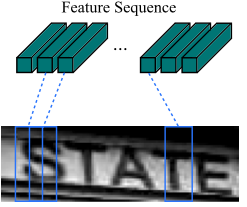
\includegraphics[width=0.3\textwidth]{img/STR-encdec-sequence-feat.png}
    \caption[Sequential feature extraction from convolution feature maps]{%
        Sequential feature extraction from convolution feature
        maps~\citep{shi_end--end_2017}\label{fig:STR-CTC-seq-feat}
    }
\end{figure}
The sequence is generated by taking column out of the feature maps from left to
right~\citep{shi_end--end_2017}.
This is possible because the parts of the feature map correspond to a spatial region of the
original image~\citep{shi_end--end_2017,goodfellow_deep_2016}.
The generated sequence features are feed into a deep \ac{BiLSTM}.
Figure~\ref{fig:bilstm} shows one layer which is made up of an \ac{LSTM} which processes the
sequence in the correct order and another \ac{LSTM} which processes the sequence
backwards~\citep{shi_end--end_2017}.
An \ac{LSTM} processed a sequence to gather context from ealier input for laterr
outputs~\citep{shi_end--end_2017,goodfellow_deep_2016}.
The \ac{BiLSTM} allows to gather context of later input for ealier outputs~\citep{shi_end--end_2017}.
This is important since a character might comprises more than one steps in the sequence
data~\citep{shi_end--end_2017}.
\begin{figure}[ht]
    \centering
    {\scriptsize%
\begin{tikzpicture}[scale=0.3]
	\node[rectangle] (Y0) at (0, 0) {$\dots$};
	\node[rectangle, draw, right=2em of Y0, minimum height=1cm, minimum width=1cm] (RNN)
        {LSTM$_\rightarrow$};
	\node[rectangle, right=of RNN, draw, minimum height=1cm, minimum width=1cm] (RNN2)
        {LSTM$_\rightarrow$};
	\node[rectangle, right=of RNN2, draw, minimum height=1cm, minimum width=1cm] (RNN3)
        {LSTM$_\rightarrow$};
	\node[rectangle, right= of RNN3, draw, minimum height=1cm, minimum width=1cm] (RNN4)
        {LSTM$_\rightarrow$};
	\node[rectangle, right=2em of RNN4] (RNN5) {$\dots$};


	\node[rectangle, above=of RNN4, draw, minimum height=1cm, minimum width=1cm] (R25)
        {LSTM$_\leftarrow$};
	\node[rectangle, left=of R25, minimum height=1cm, minimum width=1cm, draw] (R24)
        {LSTM$_\leftarrow$};
	\node[rectangle, left=of R24, draw, minimum height=1cm, minimum width=1cm] (R23)
        {LSTM$_\leftarrow$};
	\node[rectangle, left=of R23, draw, minimum height=1cm, minimum width=1cm] (R22)
        {LSTM$_\leftarrow$};
	\node[rectangle, left=2em of R22] (R21) {$\dots$};
	\node[right=2em of R25] (Y20) {$\dots$};

	\node[below=of RNN] (X1) {$\x_2$};
	\node[below=of RNN2] (X2) {$\x_3$};
	\node[below=of RNN3] (X3) {$\x_4$};
	\node[below=of RNN4] (X4) {$\x_5$};
	\node[above=of R25] (Y5) {$\h_5$};
	\node[above=of R24] (Y4) {$\h_4$};
	\node[above=of R23] (Y3) {$\h_3$};
	\node[above=of R22] (Y2) {$\h_2$};
	\node[rectangle, left=3.2em of Y2] (Y1) {$\dots$};
	\node[right=3.2em of Y5] (Y6) {$\dots$};

	\draw[-stealth] (X1) -- (RNN);
	\draw[-stealth] (X2) -- (RNN2);
	\draw[-stealth] (X3) -- (RNN3);
	\draw[-stealth] (X4) -- (RNN4);
	\draw[-stealth, densely dotted] (Y0) -- (RNN);
	\draw[-stealth] (RNN) -- node[above, pos=0.35] {} (RNN2);
	\draw[-stealth] (RNN2) -- node[above, pos=0.35] {} (RNN3);
	\draw[-stealth] (RNN3) -- node[above, pos=0.35] {} (RNN4);
	\draw[-stealth, densely dotted] (RNN4) -- (RNN5);
	\node[below=4em of Y0] (d) {\dots};
	\node[below=4em of RNN5] (d) {\dots};

	\path[-stealth, white] (X1) edge[bend left=45] (R22);
	\path[-stealth] (X1) edge[bend left=45] (R22);
	\path[-stealth, white] (X2) edge[bend left=45] (R23);
	\path[-stealth] (X2) edge[bend left=45] (R23);
	\path[-stealth, white] (X3) edge[bend left=45] (R24);
	\path[-stealth] (X3) edge[bend left=45] (R24);
	\path[-stealth, white] (X4) edge[bend left=45] (R25);
	\path[-stealth] (X4) edge[bend left=45] (R25);
	\draw[-stealth, densely dotted] (Y20) -- (R25);

	\draw[-stealth] (R22) -- (Y2);
	\draw[-stealth] (R23) -- (Y3);
	\draw[-stealth] (R24) -- (Y4);
	\draw[-stealth] (R25) -- (Y5);

	\draw[stealth-, densely dotted] (R21) -- (R22);
	\draw[stealth-] (R22) -- node[above, pos=0.65] {} (R23);
	\draw[stealth-] (R23) -- node[above, pos=0.65] {} (R24);
	\draw[stealth-] (R24) -- node[above, pos=0.65] {} (R25);
	\draw[-stealth, densely dotted] (Y20) -- (R25);

	\path[-stealth, white] (RNN) edge[bend right=45] (Y2);
	\path[-stealth] (RNN) edge[bend right=45] (Y2);
	\path[-stealth, white] (RNN2) edge[bend right=45] (Y3);
	\path[-stealth] (RNN2) edge[bend right=45] (Y3);
	\path[-stealth, white] (RNN3) edge[bend right=45] (Y4);
	\path[-stealth] (RNN3) edge[bend right=45] (Y4);
	\path[-stealth, white] (RNN4) edge[bend right=45] (Y5);
	\path[-stealth] (RNN4) edge[bend right=45] (Y5);
\end{tikzpicture}
}
%
    \caption[Bidirectional LSTM]{%
        Bidirectional LSTM~\citep{goodfellow_deep_2016}\label{fig:bilstm}
    }
\end{figure}
The generated encoded features with embedded context are then used for transcribing the final
output~\citep{shi_end--end_2017}.
The transciption uses conditional probibilities to convert the per-frame featues encoded by the
deep \ac{BiLSTM} into the label sequence which is the text instance
prediction~\citep{shi_end--end_2017}.
This process uses the conditional probabilities $p(l\|\Y)$ that are defined by~\cite{graves_connectionist_2006},
which is why the category of approaches is called \ac{CTC} based.
$l$ stands for the label sequence and \Y\ stands for the per-frame features~\citep{shi_end--end_2017}.
Each frame $\y_t$ is a probability distribution over the possible character and a `blank'
character~\citep{shi_end--end_2017,graves_connectionist_2006}.
It is distinguished between lexicon based and lexicon free transcription~\citep{shi_end--end_2017}.
Lexicon free transcription uses the most probable character or blank (-) at each frame.
\[\text{HHH-eellll-lll-\-oo-\-\-}\]
Then all duplicate characters are discarded.
\[\text{H-el-l-o}\]
At last all blanks are discarded, leaving the final prediction~\citep{shi_end--end_2017}.
\[\text{Hello}\]
For lexicon based transcription the combination of \Y\ ist checked for similarity to words in the
lexicon based on the levenstein distance (like the metrics \ac{AED}, \ac{NED} defined in
Section~\ref{se:sts})~\citep{shi_end--end_2017}.
The word in the lexicon with the largest probability to be derived from \Y\ is
chosen~\citep{shi_end--end_2017}.

For an attention based example, the approach introduced by~\cite{ghosh_visual_2017} is used.
The approach is inspired by~\cite{bahdanau_neural_2016,xu_show_2016}: It uses a \ac{CNN} for
spatial encoding of the input image which can then be used.
The attention mechanism then helps the subsequent \ac{LSTM} to choose part of the image most
important for each timestep~\citep{ghosh_visual_2017}.
\begin{figure}[h]
    \centering
    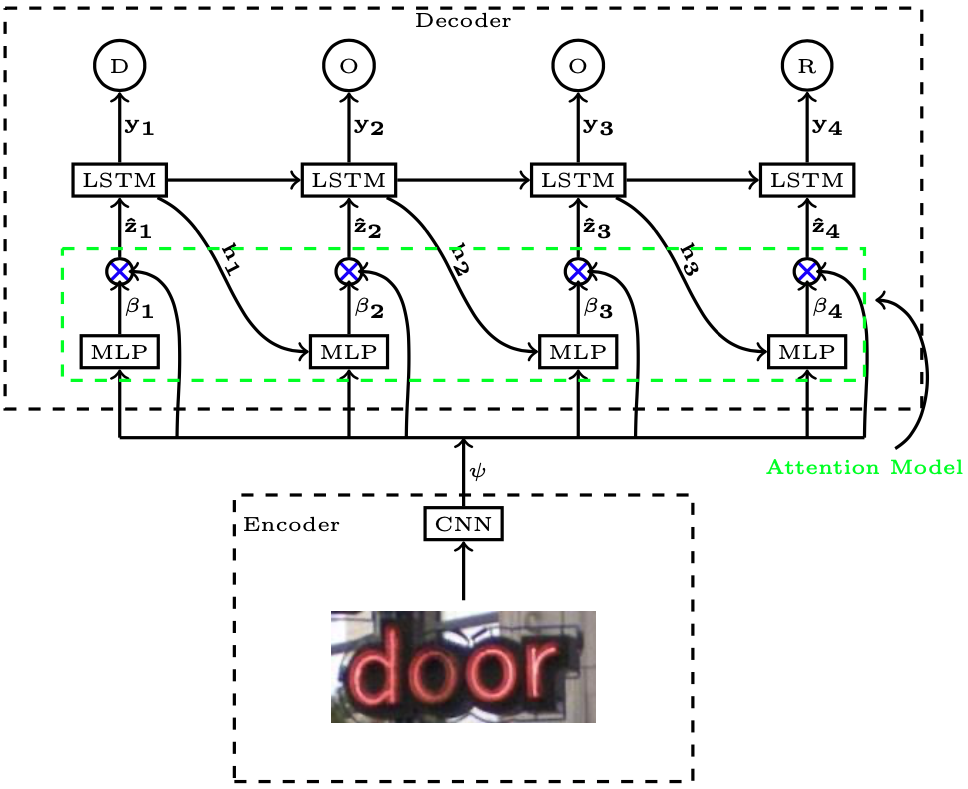
\includegraphics[width=0.7\textwidth]{img/STR-encdec-attention-Gosh-Visual-2017.png}
    \caption[Encoder decoder based STR architecture with attention mechanism]{%
        Encoder decoder based STR architecture with attention
        mechanism~\citep{ghosh_visual_2017}\label{fig:STR-attention}
    }
\end{figure}
Figure~\ref{fig:STR-attention} shows the network architecture~\citep{ghosh_visual_2017}.
The \ac{CNN} performs feature extraction and encoding~\citep{ghosh_visual_2017}.
The \ac{CNN} architecture introduced by~\cite{jaderberg_deep_2015} is used.
% FIXME: explain why this CNN
The feature map is then converted into feature vector like in
Figure~\ref{fig:STR-CTC-seq-feat}~\citep{ghosh_visual_2017,shi_end--end_2017}.
The attention mechanism is placed between the encoder \ac{CNN} and the decoder
\ac{LSTM}~\citep{ghosh_visual_2017}.



\begin{itemize}
    \item lexicon free approach
    \item adjustment of beam search algorithm for even better performance through weak explicit
        language models (prefix probabilities, not fixed lexicon)
    \item beam search to include lexicon when available
\end{itemize}


E2E
\begin{itemize}
    \item two step or two stage pipeline
    \item Bestandteile nicht zwangsweise sequentiell
\end{itemize}

\begin{table}[ht]
    \centering\scriptsize
    \begin{tabular}{p{.05\textwidth}p{.09\textwidth}p{.16\textwidth}p{.55\textwidth}}
        Task & \multicolumn{2}{c}{Approach category} & Identifying properties \\
        \toprule
        STD & Seg free & & Localize whole instances  \\
            & & 1-stage & direct \ac{BB} regression \\
            & & 2-stage & find \acp{ROI}, adjust \acp{ROI} for better fit \\
            & Seg based & & Localize sub text components to reconstruct instance \\
            & & Pixel-level & Pixel level segmentation \\
            & & Component-level & Sub-component level segmentation \\
        \midrule
        STR & Seg based & & Character segmentation and classification\\
            & Encoder Decoder based & & Sequence recognition \\
            & & CTC based & CTC rule transciption \\
            & & Attention based & Attention Mechanism \\
        \midrule
        E2E & 2 step & & Images are cropped for STR \\
            & 2 stage & & Features are cropped for STR \\
        \bottomrule
    \end{tabular}
    \caption{Tasks, method categories and identifying propertis\label{tb:steps-properties}}
\end{table}
% FIXME: after all explained: Note that mixtures of the categories are possible in practice,
%           the categorization is applied to help compare approaches (give example for mixture)

\section{State of the Art Methods}
This section documents the search for literature which provides the content for the subsequent
overview of innovation.
For this, important \ac{DL} techniques and notable advances along with their properties are researched
and presented.
For a literature review, it is important to report how the information was found and
synthesized~\citep{torraco_writing_2005}.
The strategy for researching current research is most important for a literature
review~\citep{snyder_literature_2019}.
This includes databases and keywords that were used, as well as exclusion criteria that were
enforced~\citep{torraco_writing_2005}.
The literature is identified through searching in the Google Scholar database.
The search is executed with keywords such as, but not only: Deep Learning, Text Detection,
Text Recognition, Text Spotting, Scene Text, Pipeline.
% XXX: update keywords
A criterion for further examination is an appropriate amount of citations for the piece of literature
in question.
Additionally, literature is selected through citations for and by literature which has already been
identified as important.
All research after 2018 which pertains to extracting scene text is regarded as relevant.
Standard \ac{OCR} solutions may not hold validity in practice, as the image and text conditions can
vary in the defined problem~\citep{chen_text_2021}.
The delimination from Section~\ref{se:problem} of course holds for this chapter and only literature
which concerns advances for the \ac{DL} model architecture will be regarded as important for the
scope of this thesis.
This extends to the whole pipeline from preprocessing an image to the final result of the model.
% FIXME: hierarchical graphic with found papers
% FIXME: describe proceeding
